\documentclass[border=5pt]{standalone}


\usepackage{pgfplots}
%\usepgfplotslibrary{external}
%\tikzexternalize

\begin{document}

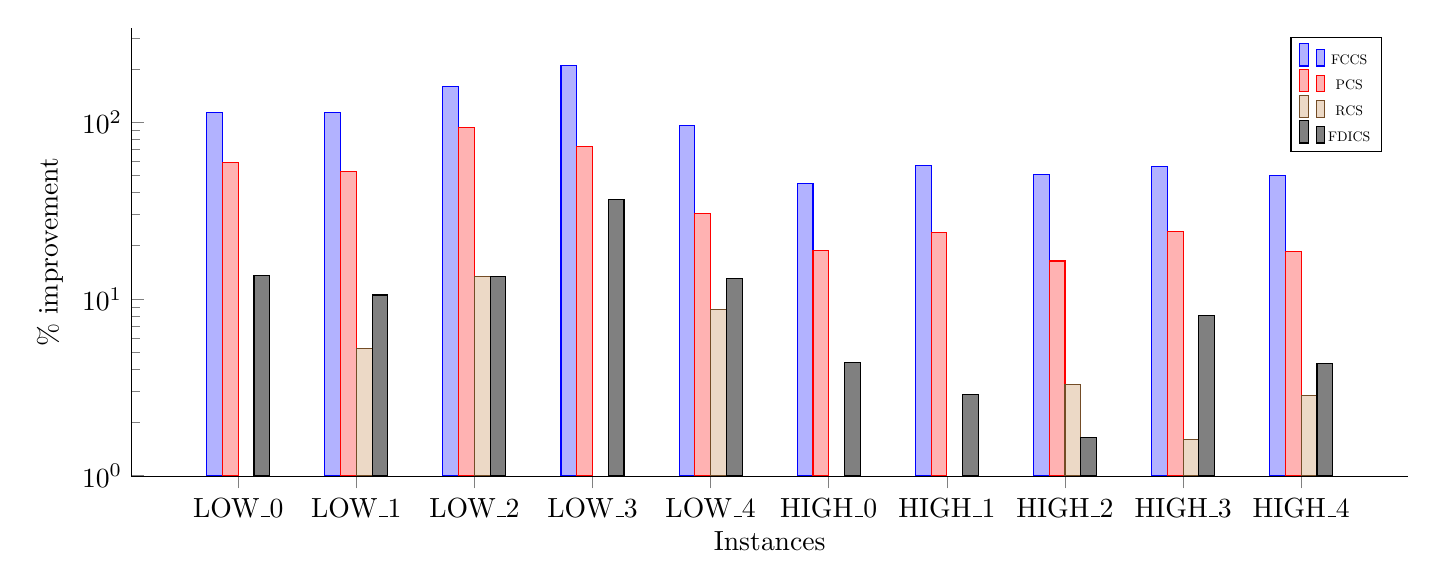
\begin{tikzpicture}
\begin{axis}[
    x tick label style={
		/pgf/number format/fixed},
    ybar=0pt,
	x=1.5cm,
	xtick=data,
    bar width=0.2cm,
    symbolic x coords={LOW\_0,LOW\_1,LOW\_2,LOW\_3,LOW\_4,HIGH\_0,HIGH\_1,HIGH\_2,HIGH\_3,HIGH\_4},
    axis lines*=left,
    ylabel = {\% improvement},
    x label style={at={(axis description cs:0.5,-0.1)},anchor=north},
    xlabel = {Instances},
    ymode = log,
    legend style={nodes={scale=0.5, transform shape}},
    ]
\addplot coordinates {(LOW\_0,113.64) (LOW\_1,113.64) (LOW\_2,160) (LOW\_3,209.09) (LOW\_4,95.65) (HIGH\_0,44.93) (HIGH\_1,56.72) (HIGH\_2,50.82) (HIGH\_3,56.45) (HIGH\_4,50)};
\addplot coordinates {(LOW\_0,59.09) (LOW\_1,52.63) (LOW\_2,93.33) (LOW\_3,72.73) (LOW\_4,30.43) (HIGH\_0,18.84) (HIGH\_1,23.88) (HIGH\_2,16.39) (HIGH\_3,24.19) (HIGH\_4,18.5)};
\addplot coordinates {(LOW\_0,0) (LOW\_1,5.26) (LOW\_2,13.33) (LOW\_3,0) (LOW\_4,8.7) (HIGH\_0,0) (HIGH\_1,0) (HIGH\_2,3.28) (HIGH\_3,1.61) (HIGH\_4,2.86)};
\addplot coordinates {(LOW\_0,13.64) (LOW\_1,10.53) (LOW\_2,13.33) (LOW\_3,36.36) (LOW\_4,13.04) (HIGH\_0,4.35) (HIGH\_1,2.89) (HIGH\_2,1.64) (HIGH\_3,8.06) (HIGH\_4,4.29)};
\legend{FCCS,PCS,RCS,FDICS}
\end{axis}
\end{tikzpicture}
\end{document}